\documentclass[11pt, oneside]{article}

% Required packages
\usepackage[letterpaper, margin=1in, includeheadfoot]{geometry}
\usepackage{hyperref}
\usepackage{tabularx}
\usepackage{lastpage}

% Header and Footer
\usepackage{fancyhdr}
\renewcommand{\headrulewidth}{1pt}
\fancypagestyle{firstpages}{ % For first few pages
\lhead{\textsc{CEE 588}}\chead{\textsc{Princeton University}}\rhead{\textsc{J.~G.~Tylka}}
\lfoot{}\cfoot{\thepage}\rfoot{}
\pagenumbering{roman}
}
\fancypagestyle{pages}{ % For all other pages
\lhead{\textsc{CEE 588}}\chead{\textsc{Princeton University}}\rhead{\textsc{J.~G.~Tylka}}
\lfoot{}\cfoot{\thepage ~of \pageref{LastPage}}\rfoot{}
\pagenumbering{arabic}
}

% Additional packages
\usepackage{graphicx}
\usepackage{subcaption}
\usepackage{amssymb}
\usepackage{amsmath}
\usepackage[numbers,square,sort]{natbib}

% User-defined commands
\newcommand{\figref}[1]{Fig.~\ref{#1}}
\newcommand{\eqnref}[1]{Eq.~(\ref{#1})}
\newcommand{\eqnreftwo}[2]{Eqs.~(\ref{#1}) and (\ref{#2})}
\newcommand{\secref}[1]{Sec.~\ref{#1}}

\renewcommand{\baselinestretch}{1.5}

\begin{document}

%%%% TITLE PAGE %%%%
\begin{titlepage}
\begin{center}
~\\[1cm]
\textsc{\LARGE Princeton University}\\[1.5cm]
\textsc{\Large CEE 588: Boundary Layer Meteorology}\\[1.5cm]
\textbf{ \Large Characterization of an Autoregressive Model for Forecasting Wind Velocity}\\[1.5cm]
{\large Joseph G.~Tylka}\\
{\large \href{mailto:josephgt@princeton.edu}{josephgt@princeton.edu}}\\
\vfill
{\large Submitted: May 19\textsuperscript{th}, 2018}
\end{center}
\end{titlepage}

\pagestyle{firstpages}
%%%% ABSTRACT %%%%
\begin{abstract}
% The first sentence should be a very succinct statement of the problem; almost a rewording of the title with a few explanatory words
An autoregressive model for forecasting wind velocity is implemented and characterized.
% The second sentence should give specific motivation for the work
Autoregression is a well-established method for short-term (intraday) time-series forecasting of wind velocity, but the performance of the model depends on the temporal characteristics of the winds.
% The following 2-3 sentences should be about the adopted method and approach
Given a time-series dataset of past wind velocities, an autocorrelation is computed and used to determine relevant timescales over which past wind velocities might be useful predictors of future data.
%Using the autocorrelation of a time-series dataset of wind velocities, relevant timescales over which past wind velocities might be useful predictors of future data are determined.
Subsequently, an autoregressive model is implemented and its performance is compared, in terms of a prediction error, to the performances of two simpler predictive models: persistence and a random sample.
Additionally, the performance of the autoregressive model is characterized by examining the dependence of the incurred prediction errors on season and on time of day.
% The rest should be a statement of all the major findings
Results of the timescale analysis suggest that the wind system will tend to ``forget'' previous wind conditions after approximately 5.5 days.
Indeed, performance results show that, while the autoregressive model consistently outperforms the alternative models, it reaches a plateau in prediction error over approximately that timescale.
The autoregressive model is also shown to yield significantly more accurate predictions in the Summer than in the Winter, and slightly more accurate predictions during the day than at night.
\end{abstract}
\newpage
\tableofcontents
\newpage
\listoffigures

% Research questions:
% Q1: what are the relevant timescales? i.e., how far into the future must one travel to "forget" about the previous wind conditions?
% Q2: how does the autoregressive model compare to persistence and random models?
% Q3: how does the performance of the autoregressive model vary with season and time of day?

\newpage
\pagestyle{pages}
%%%% INTRODUCTION %%%%
\section{Introduction}
% Motivation for work (from a very general perspective)
In order to facilitate the integration of wind energy into the power grid, reliable methods of forecasting wind power are required.
Existing forecasting methods generally take a statistical, physical, or combined approach \citep{Wang2011}.
For short-term (intraday) predictions, statistical approaches, such as direct time-series forecasting, are often preferred.
Several such methods are reviewed by \citet[Chap.~2]{Giebel2011}.
For longer-term predictions, physics-based numerical weather prediction (NWP) models are often preferred, or at least included in a combined approach, as such models have been shown to outperform time-series forecasts beyond about 6 hours ahead \citep[Sec.~1.3]{Giebel2011}.

% Review of previous work focusing on the remaining problems (questions or deficiencies) the present paper claims to contribute to solving
It is well-established that modern weather forecasting models, which tend to employ a combination of statistical and physical models, can only accurately forecast about 5--7 days into the future \citep[Sec.~1.2]{Giebel2011}.
For time-series forecasting models such as an autoregression, whose predictions draw heavily on recent data, the upper limit on how far ahead such models can accurately predict is likely related to the timescale over which the wind system ``forgets'' about previous conditions.
Consequently, the primary objective of the present work is to empirically determine this timescale and characterize the time-domain performance of an autoregressive model.

\citet{Brown1984} first proposed using an autoregressive model to forecast wind speed and power, but found that their model only yields accurate predictions up to about 3 hours ahead.
On a similar timescale, \citet{LandbergWatson1994} found that persistence models, which model future wind conditions as identical to the most recent measurement, tend to outperform their NWP model up to about 6 hours ahead.
Numerous other studies, many of which are reviewed by \citet[Sec.~2.1]{Giebel2011}, have demonstrated that autoregressive (or, more generally, autoregressive moving-average) models can be optimized to outperform persistence over most, if not all, timescales.
In view of these findings, here, we use persistence as a benchmark against which to compare the forecasting accuracy of the autoregressive model.

% A statement of the paper's main question(s) and goal(s), followed by a succinct description of the general method and approach to be described in the paper
In order to determine the timescales over which an autoregressive model can be expected to perform well, we analyze the autocorrelation of a dataset of historical wind velocities. %%TODO%% "we" vs "I"
We then implement an autoregressive model, the parameters of which (i.e., the autoregression coefficients) are computed using these same historical wind data, and evaluate it using the same dataset but for a distinct (i.e., non-overlapping) time period.
This evaluation consists of randomly selecting segments of measured wind data as an input to the model, and comparing the predictions of the model to the measured data immediately following the input segment.
The performance of the autoregressive model is then compared, over various prediction timescales, to the performances of two simpler predictive models: persistence and a random sample.
Additionally, the performance of the autoregressive model is further characterized by examining the dependence of the incurred prediction errors on season and on time of day.

% A brief section by section description of the structure of the paper
The rest of this report is organized as follows.
In \secref{sec:Theory}, we review the mathematical theory used in this work as well as several forecasting models.
Next, in \secref{sec:Methodology}, we describe the analyses conducted in order to determine relevant timescales and to characterize the performance of each forecasting model.
In \secref{sec:Results}, we present and discuss the results of these analyses, and finally,
in \secref{sec:Conclusions}, we summarize this work and draw conclusions from the results.

%%%% THEORY %%%%
\section{Review of Mathematical Theory}\label{sec:Theory}
In this section we first formulate the time-series forecasting problem.
We then review four pairwise (i.e., ``two-point'') statistics functions: the cross- and autocorrelation and cross- and autocovariance functions.
Finally, we review three forecasting models that we implement and evaluate in this work.

\subsection{Problem Formulation}
Consider the stream-wise and cross-stream wind velocities, $u(t)$ and $v(t)$, respectively, sampled at times $t_n$ for all integers $n$ with a sampling rate $F_s$, such that $t_n = n/F_s$.
For simplicity, we consider $t_n < 0$ to be the ``past'' and $t_n \geq 0$ to be the ``future.''
We write the wind velocity as a complex variable, $z(t) = u(t) + i v(t)$, where $i$ is the imaginary unit, and denote the sampled wind data by $z_n = z(t_n)$.
The goal of time-series forecasting of wind velocity is to use past wind data, say $N_\text{in}$ previous samples, to predict $N_\text{out}$ future samples.
That is, we seek a set of forecasting functions $f_n$ such that
\begin{equation}
z_n = f_n (z_{-1}, z_{-2}, \dots, z_{-N_\text{in}} ), \text{ for all } n \in [0, N_\text{out} - 1].
\end{equation}

\subsection{Pairwise Statistics Functions}
Consider two (possibly complex-valued) sequences $X_n,Y_n$, for all integers $n \in [0,N-1]$.
An unbiased estimate of the cross-correlation of these sequences is given by\footnote{See: \url{https://www.mathworks.com/help/signal/ref/xcorr.html}}
\begin{equation}\label{eq:xcorr}
R_{XY}(m) =
\begin{cases}
\displaystyle \frac{1}{N - |m|} \sum_{n=0}^{N-m-1} X_{n+m} \overline{Y_n}, & \text{for } m \geq 0,\\[20pt]
\overline{R_{XY}}(-m), & \text{for } m < 0,
\end{cases}
\end{equation}
for all integers $m \in [-(N-1),N-1]$, where $\overline{(\cdot)}$ denotes taking the complex conjugate of the argument.
Furthermore, the autocorrelation of a single sequence, $X_n$, is given by $R_{XX}(m)$.
Note that this definition differs from that given by \citet[Sec.~8.2.1]{Stull1988}, in which the mean of the sequence is removed (cf.~\eqnref{eq:xcov} below) and a different normalization is used.

Similarly, an unbiased estimate of the cross-covariance of $X_n$ and $Y_n$ is given by\footnote{See: \url{https://www.mathworks.com/help/signal/ref/xcov.html}}
\begin{equation}\label{eq:xcov}
C_{XY}(m) = 
\begin{cases}
\displaystyle \frac{1}{N - |m|} \sum_{n=0}^{N-m-1} \left( X_{n+m} - \langle X \rangle \right) \left( \overline{Y_n} - \left\langle \overline{Y} \right\rangle \right), & \text{for } m \geq 0,\\[20pt]
\overline{C_{XY}}(-m), & \text{for } m < 0,
\end{cases},
\end{equation}
where $\langle \cdot \rangle$ denotes taking the mean, i.e.,
\begin{equation}
\langle X \rangle = \frac{1}{N} \sum_{n = 0}^{N-1} X_n.
\end{equation}
Note that the cross-covariance is related to the cross-correlation by $C_{XY}(m) = R_{\delta_X \delta_Y}(m)$, where $\delta_{X_n} = X_n - \langle X \rangle$ and $\delta_{Y_n} = Y_n - \langle Y \rangle$ represent each sequence's deviation from its mean, and the autocovariance of $X_n$ is given by $C_{XX}(m) = R_{\delta_X \delta_X}(m)$.

%%%% FORECASTING MODELS %%%%
\subsection{Forecasting Models}\label{sec:Models}
In this section we review three forecasting models used in this work.
Here, we denote the measured wind velocity by $z_n$ and the predicted wind velocity by $z_n'$.

\subsubsection{Persistence}
One well-established yet inherently limited forecasting model is known as the ``persistence'' model \citep[Sec.~1.5]{Giebel2011}, wherein all future wind velocities are taken to be equal to the most recent wind velocity sample, i.e.,
\begin{equation}
z_n' = z_{-1}, \text{ for all } n \in [0, N_\text{out} - 1].
\end{equation}
Given this model's construction, we can expect (and indeed we will see in \secref{sec:Results:Comparison}) that the prediction errors incurred by this model will be small in the very short-term, but will increase rapidly with increasing time.

\subsubsection{Random Sample}
Given a database of historical wind velocities, $\zeta_m$, for all integers $m \in [0, M-1]$, we randomly select a segment of $N_\text{out}$ consecutive samples as the predicted future data.
That is, for some randomly selected integer $r \in [0, M - N_\text{out}]$, we take
\begin{equation}
z_n' = \zeta_{r+n}, \text{ for all } n \in [0, N_\text{out} - 1].
\end{equation}
For this model, we can expect (and again we will see in \secref{sec:Results:Comparison}) that the prediction errors will be large and, on average, relatively constant with time, as the randomly selected segment is likely uncorrelated with the true future data.

\subsubsection{Autoregression}\label{sec:Models:Autoregression}
An autoregressive model of order $P$ uses a linear combination of the $P$ most recent time samples to predict the following one.
In general, this can be written as
\begin{equation}
z_n' = \sum_{p = 1}^P \phi_p z_{n-p},
\end{equation}
where $\phi_p$ are the autoregression coefficients for all integers $p \in [1, P]$.
In practice, this formula is applied successively to predict $z_0'$, then $z_1'$, then $z_2'$, and so forth.
%\begin{align}
%z_0' &= \sum_{p = 1}^P \phi_p z_{-p},\\
%z_1' &= \phi_1 z_0' + \sum_{p = 2}^P \phi_p z_{1-p},\\
%z_2' &= \phi_1 z_1' + \phi_2 z_0' + \sum_{p = 3}^P \phi_p z_{2-p},
%\end{align}
Note that, in contrast to much of the existing literature, this formulation simultaneously forecasts wind speed and direction (i.e., wind velocity), whereas often only the wind speed is considered \citep[for example]{Brown1984}.

Here, we compute the autoregression coefficients using a database of historical wind data $\zeta_m$ for all integers $m \in [0, M-1]$.
According to the Yule-Walker equations and provided that $P < M$, the autoregression coefficients are given by \citep[Sec.~3.1.1]{Chatfield2000}
\begin{equation}
\begin{bmatrix}
C_{\zeta \zeta}(1) \\
C_{\zeta \zeta}(2) \\
\vdots \\
C_{\zeta \zeta}(P)
\end{bmatrix}
=
\begin{bmatrix}
C_{\zeta \zeta}(0) & C_{\zeta \zeta}(-1) & \cdots & C_{\zeta \zeta} (-P+1) \\
C_{\zeta \zeta}(1) & C_{\zeta \zeta}(0) & \cdots & C_{\zeta \zeta} (-P+2) \\
\vdots & \vdots & \ddots & \vdots \\
C_{\zeta \zeta}(P-1) & C_{\zeta \zeta}(P-2) & \cdots & C_{\zeta \zeta}(0)
\end{bmatrix}
\cdot
\begin{bmatrix}
\phi_1 \\
\phi_2 \\
\vdots \\
\phi_P
\end{bmatrix},
\end{equation}
where $C_{\zeta \zeta}$ is computed using \eqnref{eq:xcov}.

Similar to the persistence model, we can expect (and again we will see in \secref{sec:Results:Comparison}) that the prediction errors incurred by this model will be small in the very short-term, but will then increase with increasing time as the wind system ``forgets'' about the previous wind conditions.

%%%% METHODOLOGY %%%%
\section{Methodology}\label{sec:Methodology}
In this work, we use a database of wind velocity measurements from the Cabauw meteorological tower,\footnote{Available for download here: \url{http://www.cesar-database.nl/Welcome.do}} which is a 213 m tall tower that has been recording, since 1986, the horizontal wind speed and direction at several vertical heights \citep[Table I]{VanUldenWieringa1996}. 
These wind speeds and directions are measured using a combination of cup and sonic anemometers and weather vanes \citep[Sec.~2.1]{Petrovic2018}.
We perform a pairwise statistical analysis of this data to determine relevant timescales, and
subsequently, we implement and characterize the three forecasting models reviewed in \secref{sec:Models}.

As our historical ``training'' dataset, $\zeta_m$, we use the wind velocity data measured at 200 m from January 1\textsuperscript{st}, 2001, until (and including) December 31\textsuperscript{st}, 2010.
These data are given at a sampling rate of $F_s = 6$ samples per hour.
As a pre-processing step, we first determine a nominal ``average'' direction for the wind.
To do this, we compute the wind direction $\theta_m = \arg (\zeta_m)$, where $\arg ( \cdot )$ denotes taking the argument (i.e., phase angle) of a complex number, such that $\zeta_m = |\zeta_m| e^{i \theta_m}$.
We then compute a histogram of these $\theta_m$, with a bin width of $3^\circ$, and subsequently find the peak of this histogram, which, for these data, occurs at $\hat{\theta} = -130.5^\circ$. %%TODO%% what is 0^\circ?
We then realign the training dataset and all other wind data used hereafter by computing
\begin{equation}
\hat{\zeta}_m = \zeta_m e^{-i\hat{\theta}}
\quad\quad \text{and} \quad\quad
\hat{z}_n = z_n e^{-i\hat{\theta}}.
\end{equation}

\subsection{Timescale Analysis}\label{sec:Methodology:Timescale}
In order to determine the timescales over which an autoregressive model can be expected to perform well, we compute the autocorrelations of both $U_m$ and $V_m$, where $\zeta_m = U_m + i V_m$.
From these autocorrelation sequences, we define an integral timescale, $T_X$ (where $X$ can be replaced by either $U$ or $V$), given by \citep{ONeill2004}
\begin{equation}\label{eq:Timescale}
T_X = \sum_{m = 0}^{M-1} R_{XX}(m) \Delta t,
\end{equation}
where $\Delta t = 1/F_s$.\footnote{Also see: \url{https://en.wikipedia.org/wiki/Integral_length_scale}}
However, in practice, we may choose to sum only over $M_\text{max}$ samples, where $M_\text{max} < M$ and is chosen based on when $R_{XX}$ reaches a sufficiently small value.
Here, we choose $M_\text{max}$ as the point at which $R_{XX}$ reaches its ``steady-state'' value, $\tilde{R}_{XX}$.

Note that an autocorrelation sequence may have a non-zero steady-state value when, for example, the sequence $X$ is sufficiently consistent such that its autocorrelation remains relatively constant over a wide range of $m$.
In such cases, we use a modified form of \eqnref{eq:Timescale}, such that $T_X$ is given by
\begin{equation}\label{eq:Timescale_mod}
T_X \approx \frac{1}{1 - \tilde{R}_{XX}} \sum_{m = 0}^{M_\text{max}-1} (R_{XX}(m) - \tilde{R}_{XX}) \Delta t.
\end{equation}
Note that if $\tilde{R}_{XX} = 0$, then \eqnref{eq:Timescale_mod} reduces to the unmodified \eqnref{eq:Timescale}.

\subsection{Performance Characterization}
In order to characterize the performance of the autoregressive model, we first compare its performance to the performances of the other forecasting models reviewed in \secref{sec:Models}.
Subsequently, we investigate the dependence of the prediction errors incurred by the autoregressive model on season and on time of day.

\subsubsection{Comparison of Forecasting Models}\label{sec:Methodology:Comparison}
For each of the forecasting models reviewed in \secref{sec:Models}, we compute an incurred prediction error.
To do this, we randomly select test segments of measured wind data from an ``evaluation'' dataset, for which we use the Cabauw wind data from January 1\textsuperscript{st}, 2011, until (and including) December 31\textsuperscript{st}, 2017.
Each test segment is $N_\text{in} + N_\text{out}$ samples long, where the first $N_\text{in}$ samples are given as an input to each model, and the following $N_\text{out}$ samples serve as a reference against which each model's prediction is compared.
We then compute the prediction error, $\epsilon_n = z_n - z_n'$, for all integers $n \in [0,N_\text{out}-1]$, where $z_n$ and $z_n'$ are the true (reference) and predicted wind velocities, respectively.

We perform this calculation for $Q$ randomly selected test segments, and compute the root-mean-square (RMS) magnitude error over all test segments, given by
\begin{equation}\label{eq:RMSE}
\overline{\epsilon}_n = \sqrt{ \frac{1}{Q} \sum_{q = 1}^Q \left| \epsilon_n^{(q)} \right|^2 },
\end{equation}
where $\epsilon_n^{(q)}$ is the prediction error for the $q^\text{th}$ test segment.

\subsubsection{Dependence on Season and on Time of Day}\label{sec:Methodology:SeasonalAndDiurnalDependence}
To investigate the seasonal dependence of the prediction errors, we repeat a very similar analysis to that described above in \secref{sec:Methodology:Comparison}, but restrict the randomly selected test segments to be from a given season.
In particular, we ensure that the entire test segment is contained within the same season.
Here, we use ``Winter'' to refer to December through February;
``Spring'' refers to March through May;
``Summer'' refers to June through August; and
``Fall'' refers to September through November.
Similarly, to investigate the dependence on the time of day, we restrict the randomly selected test segments such that the reference wind velocity segments are no longer than 12 hours and are either ``daytime'' (starting at 8AM) or ``nighttime'' (starting at 8PM) segments.

%%%% RESULTS %%%%
\section{Results and Discussion}\label{sec:Results}
In this section we present and discuss the results of the analyses described above.

\subsection{Timescale Analysis}\label{sec:Results:Timescale}
In \figref{fig:Autocorrelations}, we plot the autocorrelation sequences $R_{UU}(m)$ and $R_{VV}(m)$ (for the stream-wise and cross-stream wind components, respectively), which have been normalized such that $R_{UU}(0) = R_{VV}(0) = 1$.
By averaging over the widest ``flat'' portion of each sequence, the ``steady-state'' values of these sequences are found to be approximately $\tilde{R}_{UU} = 0.1$ and $\tilde{R}_{VV} = 0$.
From the plot, we see that $R_{UU}$ reaches its steady-state value after approximately 70 days,
while $R_{VV}$ reaches its steady-state value after only approximately 15 days.
Choosing $M_\text{max}$ as the first (i.e., smallest positive) value of $m$ at which $R_{XX}(m) < \tilde{R}_{XX}$, we compute, using \eqnref{eq:Timescale_mod}, the timescales $T_U$ and $T_V$.
For each curve in \figref{fig:Autocorrelations}, the area between $\tilde{R}_{XX}$ and $R_{XX}(m)$ is shaded for $m < M_\text{max}$, representing the value of the summation in \eqnref{eq:Timescale_mod}.

\begin{figure}[htb]
\centering
\includegraphics[width=0.7\columnwidth]{figures/AutocorrelationSequences_100days}
\caption{Normalized autocorrelation sequences $R_{UU}$ (blue curve) and $R_{VV}$ (red).
The filled regions correspond to the summations computed in \eqnref{eq:Timescale_mod} to find the integral timescales $T_U$ and $T_V$.}
\label{fig:Autocorrelations}
\end{figure}

For these data, we find that the timescales computed via \eqnref{eq:Timescale_mod} are $T_U \approx 5.44$ days and $T_V \approx 1.71$ days.
These values suggest that the stream-wise winds tend to remain correlated for $\sim 5.5$ days, while the cross-stream winds remain correlated for only $\sim 2$ days.
Consequently, we can expect the errors incurred by the autoregressive and persistence models to attain relatively constant values after $\sim 5.5$ days, since, after that time, the wind conditions are essentially uncorrelated with the previous ones.
This timescale corresponds well with the previously mentioned limitation of modern weather forecasting models, which are only able to accurately forecast about 5--7 days into the future \citep[Sec.~1.2]{Giebel2011}.

\subsection{Performance Characterization}
Here, we construct an autoregressive model, as described in \secref{sec:Models:Autoregression}, with an order $P$ corresponding to 2 days, i.e., $P = 2 \times 24 F_s$, where $F_s$ is given in samples per hour.
In each analysis below, we take $N_\text{in} = 2 \times 24 F_s$ input samples and we compute, using \eqnref{eq:RMSE}, the RMS error over $Q = 100$ test segments.

\subsubsection{Comparison of Forecasting Models}\label{sec:Results:Comparison}
The RMS prediction errors incurred by each forecasting model are plotted in \figref{fig:ComparisonRMSE:12hrs} for a forecast duration of 12 hours (i.e., $N_\text{out} = 12 F_s$).
From this plot, we see that the autoregressive model performs comparably to, if not slightly better than, persistence over almost the entire forecast duration.
As expected, we see that the RMS errors incurred by the random sample model are approximately constant with time.

\begin{figure}[htb]
\centering
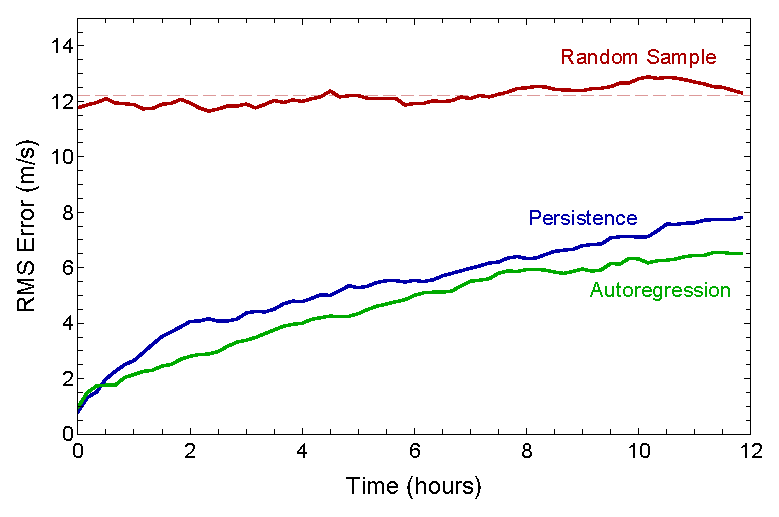
\includegraphics[width=0.7\columnwidth]{figures/ComparisonRMSPredictionError_12hrs}
\caption{Comparison of RMS prediction errors incurred by the persistence (blue curve), random sample (red), and autoregressive (green) models for predictions up to 12 hours.
The horizontal dashed red line indicates the average (mean) value of the RMS error for the random sample model (equal to approximately 12.5 m/s).}
\label{fig:ComparisonRMSE:12hrs}
\end{figure}

In \figref{fig:ComparisonRMSE:30days}, we again plot the RMS prediction errors incurred by each model, now for a forecast duration of 30 days (i.e., $N_\text{out} = 30 \times 24 F_s$).
From this plot, we see that, beyond about 1 day, the autoregressive model consistently outperforms persistence.
Additionally, we see that the errors incurred by the persistence model are small at small $t_n$, but ultimately reach similar values to those incurred by the random sample model.
We interpret this behavior as corresponding to the system ``forgetting'' about the previous wind conditions, and, in particular, we see that this happens when $t_n \approx T_U \sim 5.5$ days.

\begin{figure}[htb]
\centering
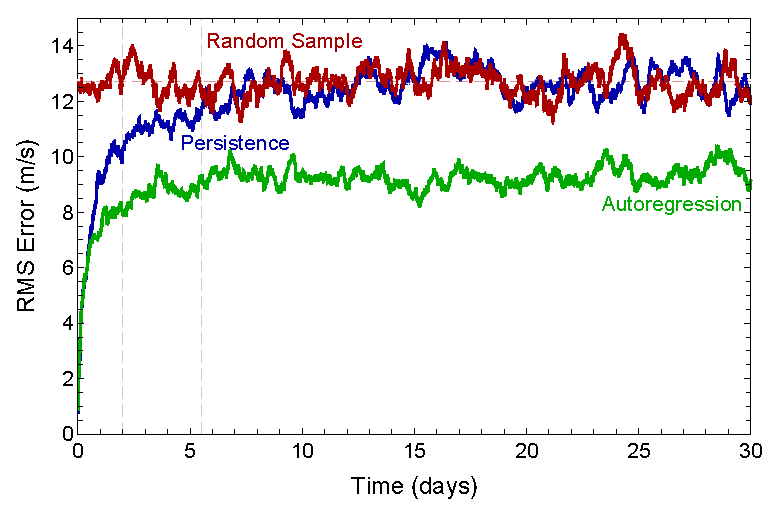
\includegraphics[width=0.7\columnwidth]{figures/ComparisonRMSPredictionError_30days}
\caption{Comparison of RMS prediction errors incurred by each model for predictions up to 30 days.
The vertical dashed lines indicate 2 and 5.5 days.
See \figref{fig:ComparisonRMSE:12hrs} for more details.}
\label{fig:ComparisonRMSE:30days}
\end{figure}

Similarly, we see that the autoregressive model reaches a plateau in RMS error beyond $T_U$.
However, these errors are still smaller than those of the persistence and random sample models.
This suggests that, even though the system has ``forgotten'' about the previous wind conditions, the autoregressive model is still able to achieve predictions that are, on average, slightly more accurate than the totally independent predictions produced by the alternative models.
As shown in \figref{fig:ComparisonRMSE:365days}, these plateaus remain constant even when forecasting up to 365 days into the future (i.e., $N_\text{out} = 365 \times 24 F_s$).

\begin{figure}[htb]
\centering
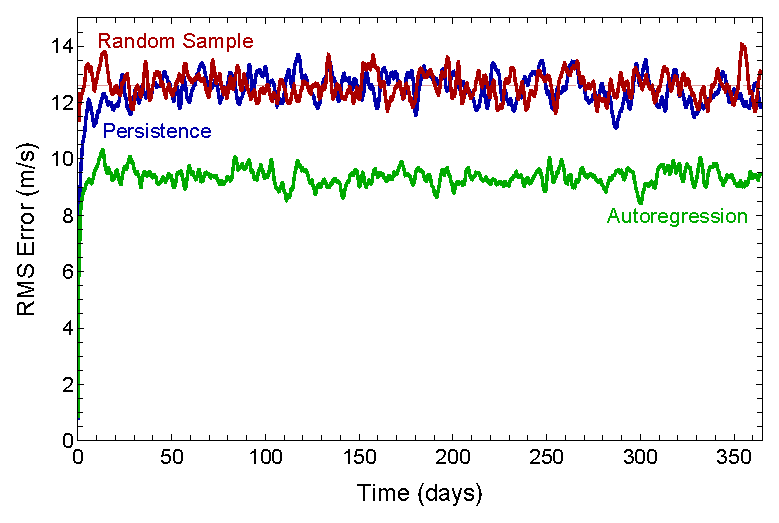
\includegraphics[width=0.7\columnwidth]{figures/ComparisonRMSPredictionError_365days}
\caption{Comparison of RMS prediction errors incurred by each model for predictions up to 365 days.
For clarity, the data have been smoothed by computing a 48-hour moving average.
See \figref{fig:ComparisonRMSE:12hrs} for more details.}
\label{fig:ComparisonRMSE:365days}
\end{figure}

\subsubsection{Dependence on Season and on Time of Day}
The RMS prediction errors incurred in each season by the autoregressive model are plotted in \figref{fig:SeasonalRMSE}.
From this plot, we see that the errors are smallest in the Summer and largest in the Winter.
This suggests that wind conditions in Spring and Summer tend to be ``more predictable'' than those in Fall or Winter.
Recall that the model coefficients used here were computed using 10 years of continuous data (see 
\secref{sec:Methodology}), which likely yielded ``average'' model coefficients that are generally suitable for all seasons, but not ideal for any season.
Consequently, that there exists a significant seasonal dependence in the observed errors suggests that one approach to reduce these errors might be to compute and employ different model coefficients for each season.

\begin{figure}[htb]
\centering
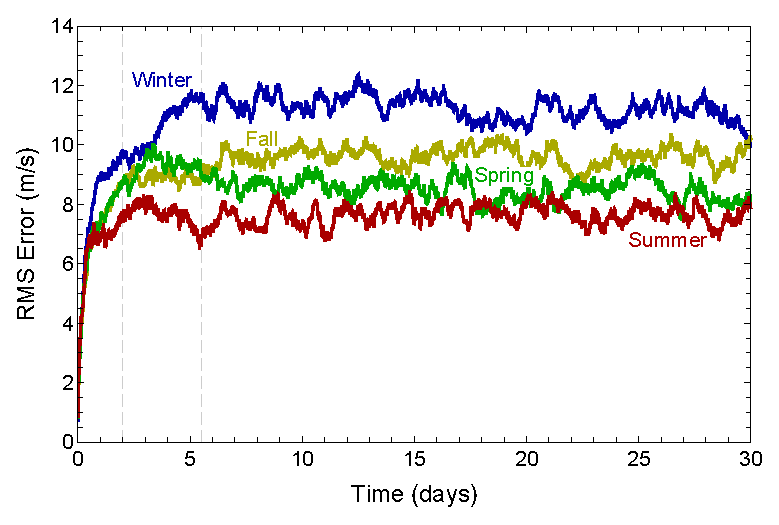
\includegraphics[width=0.7\columnwidth]{figures/SeasonalRMSPredictionError}
\caption{Prediction errors incurred by the autoregressive model in each season.
The vertical dashed lines indicate 2 and 5.5 days.
Here, ``Winter'' (blue curve) refers to December through February;
``Spring'' (green) refers to March through May;
``Summer'' (red) refers to June through August; and
``Fall'' (yellow) refers to September through November.}
\label{fig:SeasonalRMSE}
\end{figure}

The RMS prediction errors incurred under daytime and nighttime conditions by the autoregressive model are plotted in \figref{fig:DiurnalRMSE}.
From this plot, we see that the prediction errors incurred during the day are usually slightly smaller than those incurred at night.
This is somewhat surprising, as we might expect nighttime conditions to be ``more predictable'' due to the stability of the atmospheric boundary layer \citep[Fig.~1.7]{Stull1988}.
However, these results suggest that the autoregressive model may be better able to predict daytime wind conditions given data from the previous night, than it is to predict nighttime wind conditions given data from the previous day.

\begin{figure}[htb]
\centering
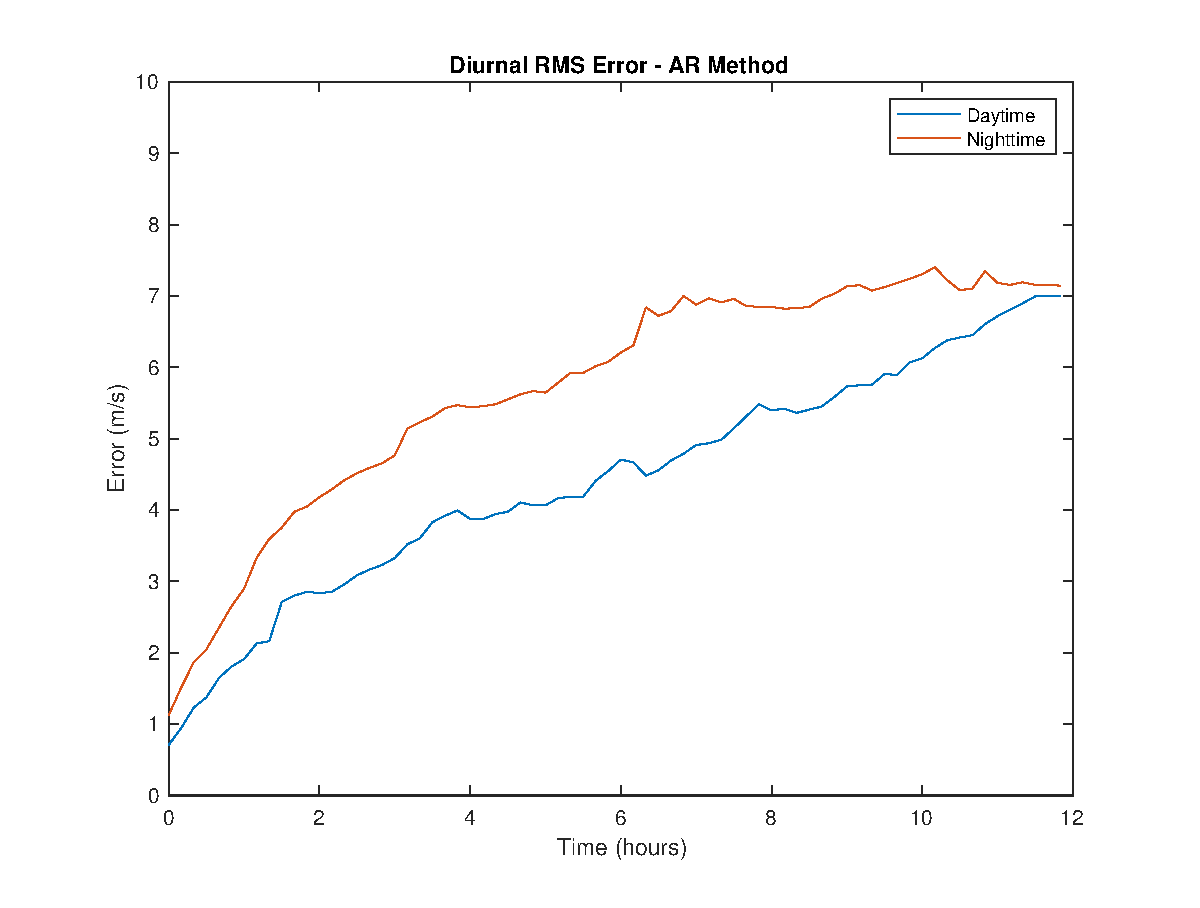
\includegraphics[width=0.7\columnwidth]{figures/DiurnalRMSPredictionError}
\caption{Prediction errors incurred by the autoregressive model under daytime and nighttime conditions.
For daytime predictions (red curve), $t = 0$ corresponds to 8AM, while for nighttime predictions (blue), $t = 0$ corresponds to 8PM.}
\label{fig:DiurnalRMSE}
\end{figure}

%%%% CONCLUSIONS %%%%
\section{Summary and Conclusions}\label{sec:Conclusions}
In this work we implemented and characterized the performance of an autoregressive model for wind velocity forecasting.
We first determined the relevant timescales over which an autoregressive model can be expected to perform well by analyzing the autocorrelation of a dataset of historical wind data.
Subsequently, we compared, over various timescales and in terms of an RMS prediction error, the performance of the autoregressive model to the performances of two simpler predictive models: persistence and a random sample.
Additionally, we examined the dependence of the incurred prediction errors on season and on time of day.

Results of the timescale analysis suggest that the wind system will tend to ``forget'' previous wind conditions after approximately 5.5 days (see \secref{sec:Results:Timescale}).
Indeed, results show that, while the autoregressive model consistently outperforms the simpler alternative models, it reaches a plateau in prediction error over approximately that timescale (see \figref{fig:ComparisonRMSE:30days}).
The autoregressive model was also found to yield more accurate predictions in the Summer than in the Winter (see \figref{fig:SeasonalRMSE}), which suggests that wind conditions in the Summer may be more consistent and ``predictable'' as a result.
Daytime predictions of wind velocity were also found to be slightly more accurate than nighttime predictions (see \figref{fig:DiurnalRMSE}), although this discrepancy does not appear to be significant.

\subsection{Future Work}
Future investigations should include an implementation of more sophisticated autoregressive models.
For example, seasonal \citep[Sec.~3.1.6]{Chatfield2000} or Markov-switching \citep{AilliotMonbet2012} autoregressive approaches, in which the autoregression coefficients vary with season, can be expected to achieve improved performance under each condition.
Additionally, the performance of the autoregressive model should be compared to numerical weather prediction models, such the Weather Research and Forecasting model,\footnote{Available for download here: \url{https://www.mmm.ucar.edu/weather-research-and-forecasting-model}} which have been shown to outperform persistence beyond about 6 hours ahead \citep{Giebel2011,LandbergWatson1994}.

\addcontentsline{toc}{section}{References}
\bibliographystyle{unsrtnat}
\bibliography{refs}

\end{document}